
We know that,
\begin{align}
   P\brak{p<X<q} &= F\brak{q^{-}}-F\brak{p} \\
    P\brak{\frac{1}{4} < X < 1} &= F\brak{1^{-}}-F\brak{\frac{1}{4}} \\
    &= \frac{3}{4} - \brak{\frac{1}{4}}^{2}\\
    &= \frac{11}{16}\\
    &= 0.6875
\end{align}
\begin{figure}[!ht]
\centering
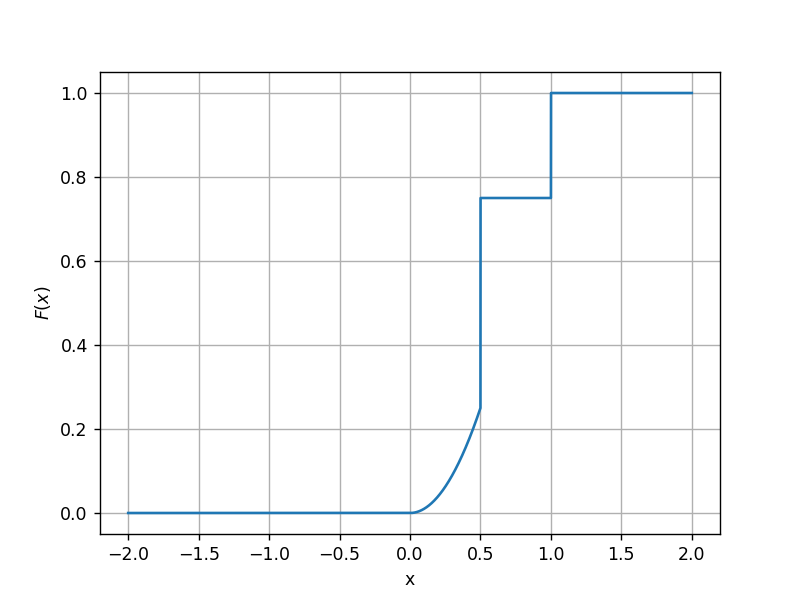
\includegraphics[width=\columnwidth]{solutions/ec/73/Assignment2.png}
\caption{The figure depicts the CDF of X}
\label{ec73:cdf}
\end{figure}

